% !TEX spellcheck = en_US

% !TEX root = expose.tex

%%%%%%%%%%%%%%%%%%%%%%%%%%%%%%%%%%%%%%%%%%%%%%%%%%%%%%%%%
\begin{frame}

\maketitle
%\vspace{1cm}
%
%\centerline{\huge \textbf{CEMRACS Project Elasto$\Phi$}}\quad\\[-5pt]
%
%\quad\\\quad\\
%
%\centerline{{\large M.~Bonazzoli$^{\dagger}$, P.~Marchand$^{*}$, X.~Claeys$^{*}$,}}
%\centerline{{\large P.-H.~Tournier$^{*}$, I.~Ben-Gharbia$^{\S}$, F.~Nataf$^{*}$}}
%
%
%\quad\\
%\hspace{2.5cm}\begin{tabular}{l}
%{\small $^{\dagger}$ Labo.~J.A.~Dieudonn\'e, Univ.~Nice Sophia Antipolis, }\\
%{\small $^{*}$  INRIA Alpines / Labo.~J.-L.~Lions UPMC,}\\
%{\small $^{\S}$ IFP Energies Nouvelles.}
%\end{tabular}
%
%
%\vspace{1cm}


%\begin{picture}(-20,10)(-10,-25)
%  \put(40,25){      
%    \put(10,-75) {
\includegraphics[height=2cm]{../logo/logo_ljll.pdf}}
%    \put(70,-75){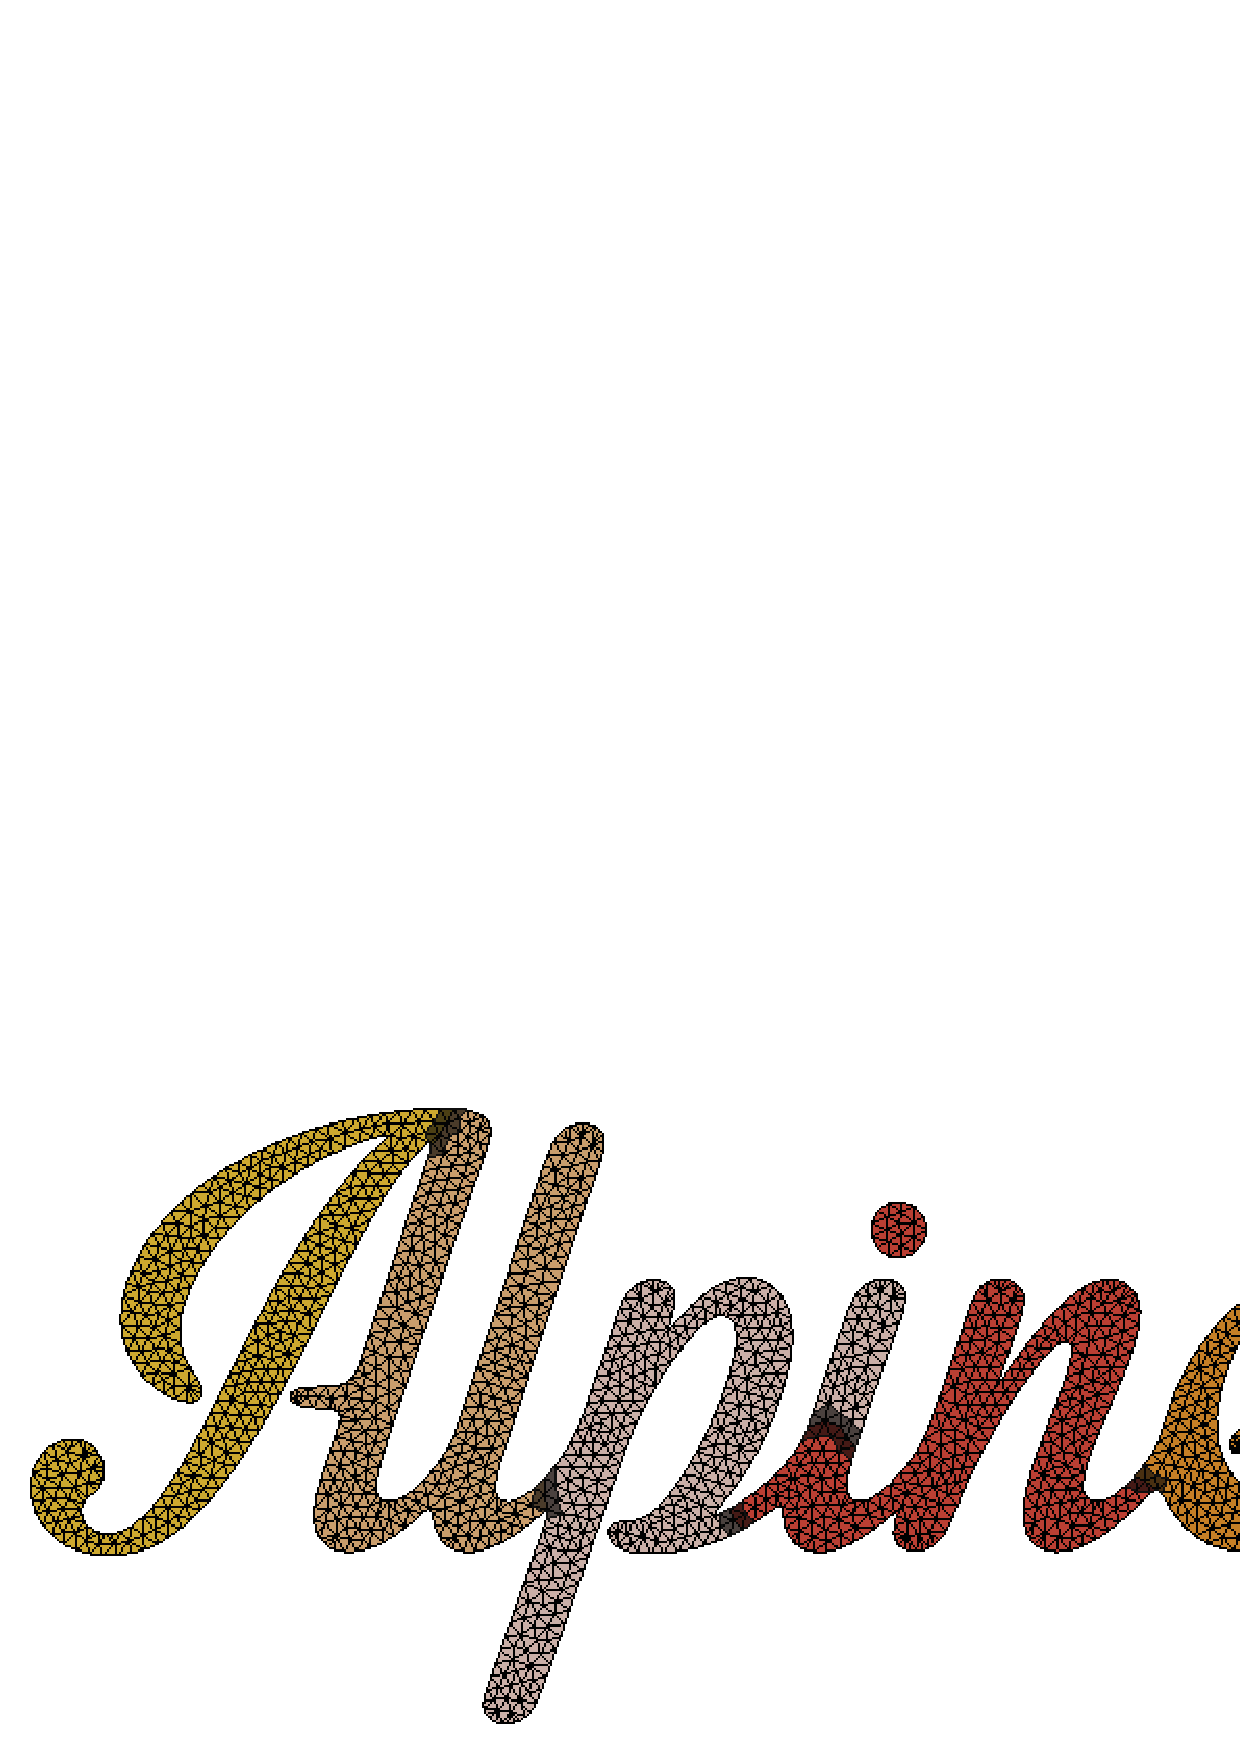
\includegraphics[height=1.75cm]{../logo/logo_alpines.pdf}}
%    \put(200,-75)  {
\includegraphics[height=2cm]{../logo/logo_anr.png}}
%    \put(10,-135)  {
\includegraphics[height=2cm]{../logo/logo_ifpen.pdf}}
%    \put(150,-135)  {
\includegraphics[height=2cm]{../logo/logo_unice.png}}
%  }
%\end{picture}

\end{frame}

%%%

\begin{frame}
\frametitle{The Elasto$\Phi$ project: the IFPEN problem} 
%\framesubtitle{}

Elastostatic problem in \alert{crack networks} of 2 types: 

geological \emph{fault} network and discrete \emph{fracture} network 

\vspace{-5pt}

\begin{figure}
\centering
\includegraphics[width=0.35\textwidth]{../images/visu_maillage5364FracsTriangles.png} \quad
\includegraphics[width=0.25\textwidth]{../images/visu_maillage1994Fracs.png}
\end{figure}

Boundary \emph{integral equation} posed at the surface of cracks

$\Rightarrow$ \alert{dense matrix} $\mA\in \R^{n\times n}$
$\Rightarrow$ $\mathcal{O}(n^{2})$ for matrix-vector product.

\medskip
IFPEN heuristic approach to sparsify $\mA$ gives large error ($16$\%--$40$\%)

\end{frame}

%%%

\begin{frame}
\frametitle{The Elasto$\Phi$ project} 
%\framesubtitle{}

Many refined \emph{complexity reduction} techniques in current literature on boundary integral equation.

\bigskip
Two ingredients in the approach we considered: 
\begin{itemize}
\item
Adaptative Cross Approximation (\alert{ACA}),
\item
Hierarchical Matrices (\alert{HM}).
\end{itemize}

\medskip
Challenge: \emph{strongly irregular geometry!}

\bigskip
\bigskip

{\tiny
[M.~Bebendorf. Hierarchical matrices: A Means to Efficiently Solve Elliptic Boundary Value Problems, {\em Lecture Notes in Computational Science and Engineering}, 2008]

\smallskip
[S.~Rjasanow, O.~Steinbach. The fast solution of boundary integral equations. {\em Mathematical and Analytical Techniques with Applications to Engineering}, 2007.]

\smallskip
[W.~Hackbusch. Hierarchical Matrices: Algorithms and Analysis, {\em Springer Series in Computational Mathematics}, 2016.]
\par} %\par per interlinea giusti

\end{frame}

%%%







